Download the zip file or tarball from \filesource.
Once downloaded, unpackage the file and open the project in the Arduino IDE\@.

If your display module's I$^2$C address is not 0x27, then edit \textit{i2c\_address.h}, and replace \lstinline{0x27} with the correct I$^2$C address for your display module.

Position both of your Cow Pi's switches in the \textit{right} position.
Connect your computer to your Cow Pi and upload the program to your Cow Pi.
The display module will show: \\
\display{
    KEY\phantom{xxx}BTN\phantom{xxx}SW \\
    \phantom{x}-\phantom{xxxx}U\phantom{x}U\phantom{xxx}R\phantom{x}R
} \\
and the right LED (the external LED) will be illuminated.
If you have the Arduino IDE's Serial Monitor open, the Serial Monitor will also show: \\
\texttt{
    KEY\phantom{xxx}BTN\phantom{xxx}SW \\
    \phantom{x}-\phantom{xxxx}U\phantom{x}U\phantom{xxx}R\phantom{x}R
}

If you forgot to place the \textbf{left switch} in the \textit{right} position, you will not have that output.
Toggle the left switch to the right and press the RESET button in the middle of the \developmentboard.
This will activate the I/O test code for this lab.

While this I/O test code is running, the display module (and the Serial Monitor) will always show the position of each of the pushbuttons (``U'' = up, ``D'' = down) and each of the switches (``L'' = left position, ``R'' = right position).
The code that determines which key (if any) on the numeric keypad is pressed will work after you write a small amount of code in Section~\ref{subsec:populatekeypad}, which the TAs will guide you through.
\textit{Do not press more than one key on the keypad at the same time.}
If both pushbuttons are pressed, then the left LED (the LED on the \developmentboard) will illuminate,
and if both switches are toggled to the right, then the right LED will illuminate.


\subsection{Description of PollingLab Files}

\subsubsection{PollingLab.ino}

Do not edit \textit{PollingLab.ino}.

This file contains the code to configure your Cow Pi for this lab and the code that determines whether to run the I/O test or the simple embedded system that you will write.

\subsubsection{i2c\_address.h}

This file exists solely to store the display module's I$^2$C address.
You do not need to edit it further.

\subsubsection{supplement.h}

Do not edit \textit{supplement.h}.

This file contains code that we hope will make it easier for you to focus on this assignment's learning objectives by taking care of a couple of the complexities.
These functions are not yet in the CowPi library but soon may be, depending on how well they work for you.

\subsubsection{io\_functions.h \& io\_functions.c}

Do not edit \textit{io\_functions.h}.

The \textit{io\_functions.c} file contains functions that you will edit in Sections~\ref{sec:LabTime} and Section~\ref{sec:MemMapIO}.
The functions that read the inputs and write to the outputs currently make use of CowPi library functions.
Your task will be to replace those library calls with code that uses the microcontroller's memory-mapped I/O registers.

\subsubsection{number\_builder.h \& number\_builder.c}

Do not edit \textit{number\_builder.h}.

The \textit{io\_functions.c} file contains a function, \function{build_number()}, that the driver code will call when you are not running the I/O test.
Right now that function is only a stub.
In Section~\ref{sec:SimpleSystem}, you will write code in \function{build_number()} (and in helper functions of your devising) to implement a simple system's specification.


\subsection{Variable Modifiers}

C has some keywords that can be used to modify variables.
In some cases, these keywords define scoping rules;
in other cases, these keywords provide information to the compiler that it can use when optimizing the resulting assembly code.

\subsubsection{const}

In LinkedListLab, you encountered the \lstinline{const} keyword.
When used as part of an ordinary variable declaration, it prevents the variable from being modified after it has been initialized.
(Much to some peoples' surprise, this does not actually make it a constant as far as C's syntax rules are concerned.)

When used with a pointer, the \lstinline{const} keyword tells the compiler that it can make optimizations under the assumption that whatever the pointer points to will not change.
Code that breaks this promise will have compile-time warnings, but it will compile and run -- but it often will have runtime errors.
(There is another way to use \lstinline{const} with a pointer that declares the pointer itself to be unchanging.)

\subsubsection{volatile}

In DuplicatorLab, you encountered the \lstinline{volatile} keyword.
A \lstinline{volatile} variable is the opposite of a \lstinline{const} variable:
not only can it change, it can spontaneously change.
The \lstinline{volatile} keyword tells the compiler that it cannot optimize-away a variable that is never written to.
It also tells the compiler that it cannot optimize-away a variable that is never read.

With threaded code such as what you saw in DuplicatorLab, it's tempting to believe that a sufficiently thorough static analysis of the code will reveal that a variable is being written to and/or read from multiple threads.
When working with memory-mapped input/output registers in this lab, you will read from variables that do not have a single line of code \textit{anywhere} changing their values, and yet their values will change.
Similarly, you will write to variables that do not have a single line of code anywhere that reads from them, and yet it is important that those variables be updated.

\subsubsection{static}

The other modifier you will see in this lab is the \lstinline{static} keyword.
If you've programmed in Java, beware that C's \lstinline{static} keyword is not the same as Java's \lstinline{static} keyword.\footnote{
    Nor can it be.
    Java's \lstinline{static} keyword declares a field to belong to the whole class;
    C does not have classes.
}

\paragraph{Static global variables}

When used with a global variable, the \lstinline{static} keyword limits that variable's scope to code to the .c file it's declared in (or to the .c file that \lstinline{#include}s the .h file it's declared in).
This allows other code in \textit{other} files to have variables with the same name without a naming collision.
That is, it makes a global variable a little less global.

\paragraph{Static local variables}

When used with a scope-limited variable, such as a variable declared in a function, the variable becomes something of a hybrid variable.
Unlike a normal function-local variable, which is allocated on the program stack, these \lstinline{static} variables are allocated on the heap.
When a function returns, normal function-local variables are deallocated because the function's stack frame is popped.
A \lstinline{static} variable, however, is \textit{not} deallocated when its function returns.
That means that its last value is still available the next time that the function is called.
A \lstinline{static} variable used in this way looks like a global variable -- its value is preserved between function calls -- but it is still scope-limited to the function it's declared in.

You can see examples of \lstinline{static} variables in the I/O test code in \textit{PollingLab.ino} and in the debouncing code in \textit{supplement.h}.

You should explicitly initialize a \lstinline{static} variable on the same line that it is declared.
Such an initializer must be a syntactic constant.
The variable will only be initialized once; it will \textit{not} be reinitialized each time the function is called.
(If it were reinitialized, that would rather defeat the point of the variable preserving its value between function calls, right?)
If you do not explicitly initialize the variable then, unlike ordinary function-local variables, a \lstinline{static} variable will automatically be initialized to 0.

If you have questions about \lstinline{static} variables, please ask the professor or a TA.
You are not \textit{required} to use \lstinline{static} variables, but it is a good idea to do so because the alternative is introducing more global variables than you might otherwise need.

\paragraph{Static array sizes}

The other use of the \lstinline{static} keyword can be seen in the first parameter for \function{display_string()} function in \textit{supplement.h}.
\begin{lstlisting}
    static inline void display_string(
        const char string[static (NUMBER_OF_DISPLAYABLE_COLUMNS+1)],
        enum row_names row
    )
\end{lstlisting}
%A array function parameter is simply a pointer.
%It normally makes no difference whether we declare the parameter as
%\begin{lstlisting}
%    const char *string
%\end{lstlisting}
%as
%\begin{lstlisting}
%    const char string[]
%\end{lstlisting}
%or as
%\begin{lstlisting}
%    const char string[NUMBER_OF_DISPLAYABLE_COLUMNS+1]
%\end{lstlisting}
%In all three cases, it's simply a pointer to a constant array.
%Even in the last case, identifying the number of elements that we expect to be in the array has no effect on the generated assembly code.
%
%Of course, here the \lstinline{const} keyword isn't an enforced requirement (if the function modifies the string, the compiler will ``only'' issue a warning, and your program will probably not work right).
%The \lstinline{const} keyword tells the compiler that it can assume the string is constant and optimize the generated assembly code accordingly.
%It also tells anyone calling the function that they can assume that the function won't change the string's characters.
%
%The \lstinline{static} keyword in \textit{this} usage serves a similar purpose.
%\begin{lstlisting}
%    const char string[static (NUMBER_OF_DISPLAYABLE_COLUMNS+1)]
%\end{lstlisting}
The \lstinline{static} keyword as used here tells the compiler that it can assume that enough memory has been allocated for at least 17 characters (including the terminating NUL character).
%This is not an enforced requirement: if you do not allocate at least 17 bytes for the string then the program will still compile but probably won't work right.
%The \lstinline{static} keyword gives the compiler permission to make optimizations that assume at least a certain number of elements are in the array.
It also tells anyone calling the function that they should make sure that is the case.
%
We do not anticipate you needing to use the \lstinline{static} keyword in this fashion;
however, because you will call \function{display_string()}, you should make sure that you call it only with strings that have at least 17 characters allocated.
(This should make sense to you, since this function is used to display a 16-character row on the display module.)


\subsection{Debouncing} \label{subsec:debouncing}

\begin{figure}[h]
    \centering
    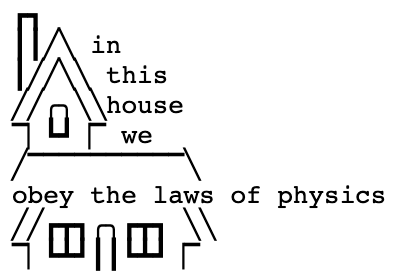
\includegraphics[height=3.5cm]{in-this-house}
\end{figure}

Mechanical buttons and switches demonstrate a phenomenon called \textit{switch bounce}.
This causes voltage to fluctuate for hundreds, often thousands, of microseconds when the contacts close or open.
When this fluctuation is in the indeterminate region between the logical low and high thresholds, it can cause the logic level to ``bounce'' back-and-forth between high and low until settling into the final, correct logic level.
This causes the digital circuitry or software to ``see'' multiple triggering events.

%A traditional way to debounce is to introduce a simple low-pass filter using a resistor and a capacitor.
%Other common hardware-based approaches use digital feedback circuits.

%Hardware design can be simplified by solving a hardware problem with software, and so you will often see hobby projects with ``debouncing code'' such as \lstinline{delay(20);} that pauses execution between detecting the first change of the button's or switch's position and acting upon it for 20ms, which should be ample time for switch bounce to stabilize.
%A problem (beyond \function{delay()} being disallowed in this lab) is that 20ms is a long time to leave your system completely non-responsive.
%
%A better solution is to continue to record the system time when a button is actually pressed or a switch is actually toggled and the device's position after that ``true action.''
%When the button or switch is polled, if fewer than 20ms have passed then ignore the actual device and report the position that resulted from the last true action.
%If more than 20ms have passed then check the device, then report the device's actual position (and also record the system time and the device's position).
%This solution allows your system to continue to respond to other external events.
%For example, you can press both buttons at very nearly the same time (or, unlikely, at the exact same time) and the software will react to both immediately.
%
%The non-blocking solution just described usually works.
%Most switch bounce finishes in under a millisecond.
%Switch bounce almost always finishes in under ten milliseconds.
%Whether using a blocking or non-blocking solution, 20ms should be ample time for a device to stop bouncing.
%We have found that some batches of the pushbuttons, slide-switches, and keypads that are included in the class kit are particularly ``dirty,'' and we have measured switch bounce sometimes lasting longer than 20ms, sometimes upwards of 150ms.
%(This happens very rarely, but often enough that we're confident it wasn't a measurement error.)
%
%The \textit{supplement.h} file includes a \function{debounce_byte()} function that takes a more-elaborate approach of reporting an input device's last ``good value'' until 20ms after the last detected bounce.
%No matter how long the device bounces, the ``time since last bounce'' resets.
%In this manner, we can be sure that bouncing has stabilized before trusting a new value found on the device.
%
%The functions in \textit{io\_functions.c} make use of \function{debounce_byte()}.
%When you modify these functions, as long as you preserve those \function{debounce_byte()} calls, you do not need to worry further about debouncing.

A traditional way to debounce is to introduce a simple low-pass filter using a resistor and a capacitor.
Other common hardware-based approaches use digital feedback circuits.
Hardware design can be simplified, and manufacturing cost can be reduced, by solving a hardware problem with software.
This, of course, transfers the design complexity to the software.

The \textit{supplement.h} file includes a \function{debounce_byte()} function that essentially implements a low-pass filter in software.
The functions in \textit{io\_functions.c} make use of \function{debounce_byte()}.
When you modify these functions, as long as you preserve those \function{debounce_byte()} calls, you do not need to worry further about debouncing.
